%
% Complete documentation on the extended LaTeX markup used for Insight
% documentation is available in ``Documenting Insight'', which is part
% of the standard documentation for Insight.  It may be found online
% at:
%
%     http://www.itk.org/

\documentclass{InsightArticle}

\usepackage[dvips]{graphicx}

%%%%%%%%%%%%%%%%%%%%%%%%%%%%%%%%%%%%%%%%%%%%%%%%%%%%%%%%%%%%%%%%%%
%
%  hyperref should be the last package to be loaded.
%
%%%%%%%%%%%%%%%%%%%%%%%%%%%%%%%%%%%%%%%%%%%%%%%%%%%%%%%%%%%%%%%%%%
\usepackage[dvips,
bookmarks,
bookmarksopen,
backref,
colorlinks,linkcolor={blue},citecolor={blue},urlcolor={blue},
]{hyperref}


%  This is a template for Papers to the Insight Journal. 
%  It is comparable to a technical report format.

% The title should be descriptive enough for people to be able to find
% the relevant document. 
\title{White Matter Stochastic Tractography}

% Increment the release number whenever significant changes are made.
% The author and/or editor can define 'significant' however they like.
\release{1.00}

% At minimum, give your name and an email address.  You can include a
% snail-mail address if you like.
\author{Tri M. Ngo$^{1}$, Carl-Fredrik Westin$^{2}$ and Polina Golland$^{3}$}
\authoraddress{$^{1}$BWH, Boston\\
               $^{2}$BWH, Boston\\
               $^{3}$MIT, Cambridge}

\begin{document}


\ifpdf
\else
   %
   % Commands for including Graphics when using latex
   % 
   \DeclareGraphicsExtensions{.eps,.jpg,.gif,.tiff,.bmp,.png}
   \DeclareGraphicsRule{.jpg}{eps}{.jpg.bb}{`convert #1 eps:-}
   \DeclareGraphicsRule{.gif}{eps}{.gif.bb}{`convert #1 eps:-}
   \DeclareGraphicsRule{.tiff}{eps}{.tiff.bb}{`convert #1 eps:-}
   \DeclareGraphicsRule{.bmp}{eps}{.bmp.bb}{`convert #1 eps:-}
   \DeclareGraphicsRule{.png}{eps}{.png.bb}{`convert #1 eps:-}
\fi


\maketitle


\ifhtml
\chapter*{Front Matter\label{front}}
\fi


% The abstract should be a paragraph or two long, and describe the
% scope of the document.
\begin{abstract}
\noindent
White matter tractography enables studies of fiber bundle characteristics.  Stochastic tractography facilitates these investigations by providing a measure of confidence regarding the inferred fiber bundles.  This article presents a multithreaded ITK stochastic tractography filter that will enable novel studies of fiber tract abnormalities.  Additionally, we provide an easy to use command line interface for the filter that is compatible with the 3D Slicer visualization environment. Finally, we demonstrate an application of the filter on real DTI images.
\end{abstract}

\tableofcontents

\section{Introduction}

\begin{figure}
\center
	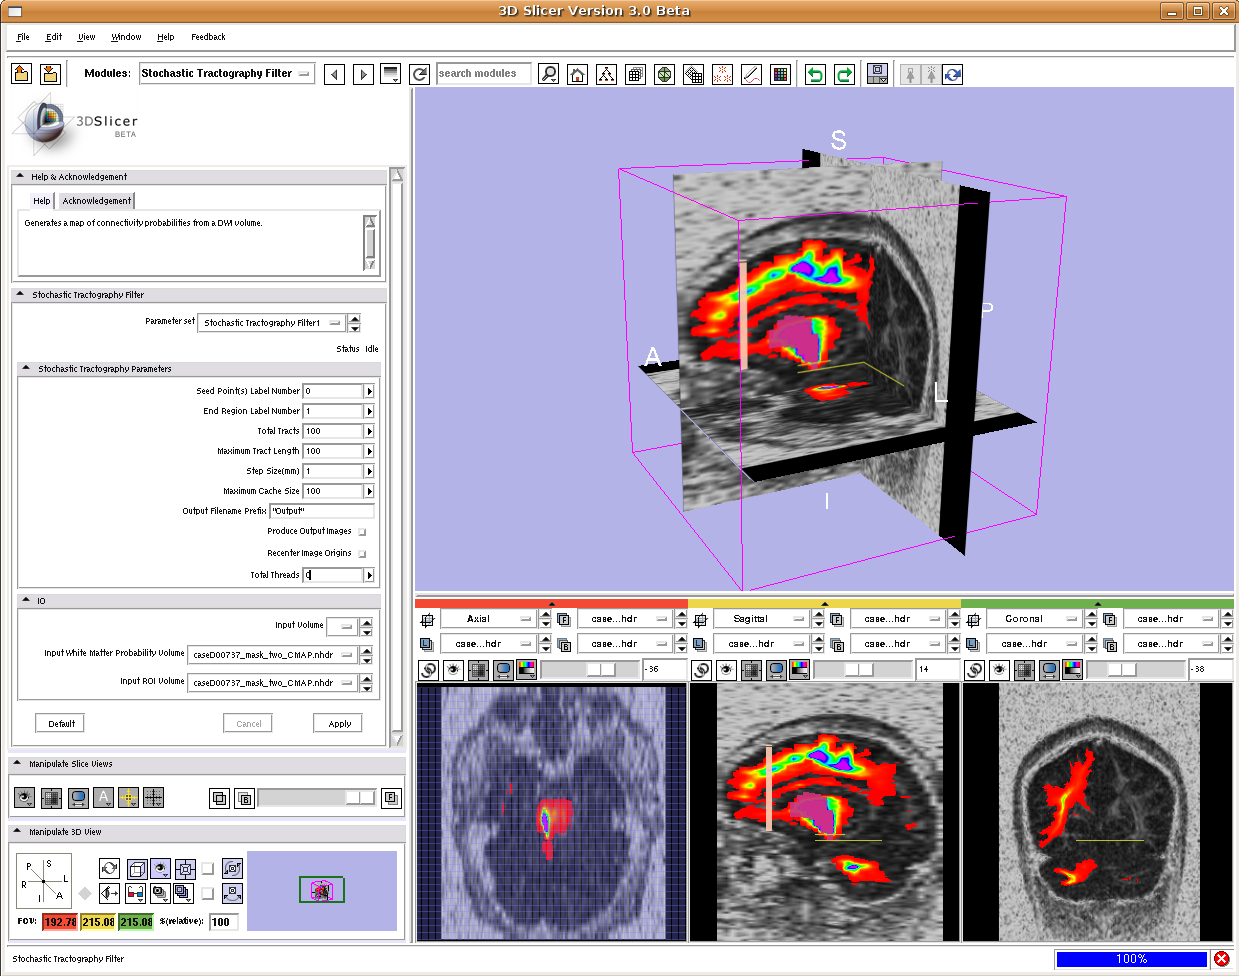
\includegraphics[width=0.75\linewidth]{slicerinterface}
	\caption{3D Slicer environment displaying the Stochastic Tractography Module interface and a connectivity map overlaid on a fractional anisotropy image.}
	\label{fig:Intro}
\end{figure}

Magnetic Resonance Imaging (MRI) is a valuable imaging modality for studying the brain in-vivo.  We can use use MRI to differentiate between tissue types, which is useful in anatomical studies.  Diffusion Tensor Imaging (DTI) provides a method to characterize white matter tracts, enabling studies of white matter architecture.

We can visualize DTI data sets using a number of methods.  DTI data sets provide information about the diffusion of water at each voxel, or volume element, in the form of diffusion tensors.  A popular technique to visualize these diffusion tensors is to extract fiber tracts which summarize the diffusion information across many voxels.  This technique is known as DTI Tractography.

One possible method of performing tractography is to generate tracts which follow the direction of maximal water diffusion of the voxels they pass through \cite{Mori99, Basser00}.  This method is known as streamline tractography.  However, this method does not provide information about the uncertainty of the generated tracks due to noise or insufficient spatial resolution.  Stochastic white matter tractography methods try to address this problem by performing tractography under a probabilistic framework.  Stochastic methods provide additional information that enables clinical researchers to perform novel studies.  Several formulations of probabilistic tractography have been suggested \cite{bjornemoMICCAI02,behrensMRM03,Tuch01,derek,Lazar05}, however tools which enable widespread adoption of stochastic tractography in clinical studies are not currently available.  This thesis implements an easy to use system for performing stochastic white matter tractography based on the algorithm described by Friman et al. \cite{frimanMICCAI05, frimanTMI06}.

Researchers have hypothesized that white matter abnormalities may underlie some neurological conditions.  For instance, people characterize schizophrenia by its behavioral symptoms.  These symptoms include auditory hallucinations, disordered thinking and delusion \cite{kubickiNYAS05}.  Studies have suggested that these behavioral symptoms have some connection with the neuroanatomical abnormalities observed in schizophrenia patients\cite{kubickiNYAS05}.  Researchers can noninvasively investigate the relationship between brain white matter abnormalities and schizophrenia by using white matter tractography.

Ultimately the success of the system developed in this thesis will depend on its use in the research community.  To this end, we implement the system within the open source ITK Segmentation and Registration Toolkit \cite{itk} framework.  ITK is currently used in many medical data processing applications.  ITK's large existing user base will encourage the system's use in the research community.  Additionally, implementing the stochastic tractography algorithm within ITK facilitates its integration into the 3D Slicer \cite{3Dslicer} for medical data visualization environment.  This thesis also implements a 3D Slicer graphical user interface module for the stochastic tractography system, increasing its ease of use and further encouraging its application in clinical research (figure \ref{fig:Intro}).

Finally, we have applied this system towards the analysis of real DTI data.  Originally, the data was investigated using non-stochastic tractography methods.  We present a new analysis of the data using the system implemented in this research.  We also compare and contrast the results obtain from stochastic tractography and non-stochastic methods.

In this thesis we describe the motivation and implementation of the stochastic tractography system followed by a demonstration of possible applications of the system.  The next chapter  provides a background on nerve fiber tracts, DTI and prior work in white matter tractography.  After the background, the following chapter provides a detailed explanation of the stochastic tractography algorithm.  Then, we describe the implementation of the algorithm within the ITK framework and optimizations used to improve performance.  Next, we demonstrate the system through an example analysis of frontal lobe nerve fiber bundles.  We conclude by discussing a potential study enabled by the algorithm.

\section{Algorithm Overview}

\begin{figure}
  \center 
	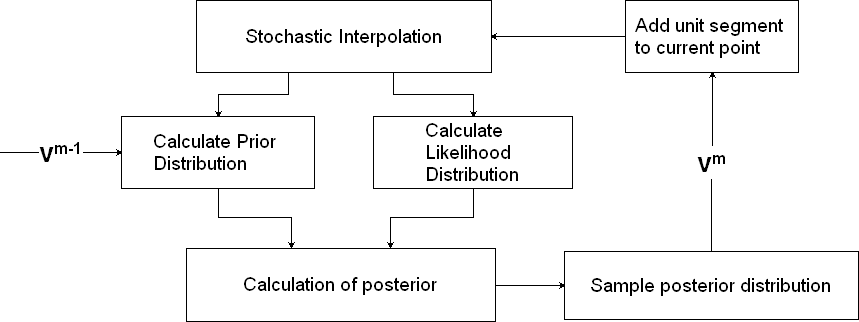
\includegraphics[width=\linewidth]{stflowsmall}
	\caption{A flow chart demonstrating key steps in the stochastic tractography algorithm}
	 \label{fig:stflow}
\end{figure}
The stochastic tractography algorithm implemented in this thesis is based on Friman's \cite{frimanTMI06} approach with some modifications to the stopping criteria.  Figure \ref{fig:stflow} provides a flow chart demonstrating key steps in the algorithm. 

A fiber tract is modeled as a sequence of unit vectors.  The orientation of these unit vectors is determined by sampling a posterior fiber orientation distribution which is dependent on the local diffusion data as well as the orientation of the unit vector in the previous step.  The posterior distribution is a normalized product of the prior likelihood of the fiber orientation and the likelihood of that fiber orientation given the local diffusion data.

Friman uses a subset of the tensor model which is called a constrained diffusion model.  In this model, the two smallest eigenvectors of diffusion tensor are equal, constraining the shape of the diffusion tensor to be linearly anisotropic.  The constrained model rules out the possibility of nonlinear, or non-cylindrical anisotropic diffusion distributions.  Deviations from linearly anisotropic diffusion distributions are captured as uncertainty in the fiber orientation.  The constrained model is combined with a Gaussian DWI noise model to obtain a fiber orientation likelihood function.  The parameters for the constrained model are derived from a weighted least squares estimation of the parameters for the log tensor model.

The orientation of each vector depends only on the previous vector.  This dependency is formulated in the prior on the fiber orientation.  Prior knowledge about the regularity of the fiber tract can encoded in this prior probability.  The prior also serves to prevent the fiber from backtracking, since the likelihood distribution alone is axially symmetric.

Friman's approach is a Bayesian inference algorithm similar to Behrens's but with some important optimizations \cite{frimanTMI06}.  In contrast with Behrens's two-compartment observation model, the constrained model used by Friman is derived from the thoroughly studied tensor model of diffusion.  The advantage of using the constrained model is that it is relatively easy to estimate the parameters for the model.  The parameters for the constrained model are obtained after the tensor model has been fit to the diffusion data.  Since the parameters for the tensor model are easily obtained through many computationally efficient ways, the constrained model's parameters are likewise easy to obtain.  The constrained model can be fit to every voxel within a matter of seconds whereas Behrens's model takes a couple of hours \cite{frimanTMI06}.  Additionally Friman avoids using MCMC techniques by assuming that parameters other than the principle diffusion direction take on their ML estimates with certainty within each voxel.  Friman demonstrates that eliminating this source of uncertainty has little effect on the resulting posterior fiber orientation distribution.

In Friman's paper on stochastic tractography, the tracking is terminated when an encountered voxel's diffusion distribution below a minimal measure of anisotropy.  However, since the stochastic tractography algorithm takes into account this uncertainty with an increase in the spatial variance of sampled fibers, this termination criterion seems arbitrary and contradictory with the goals of stochastic tractography, which is to enable sampling of tracts in regions of uncertainty.  Thus we replace this termination criterion with one which terminates tractography based on the posterior probability that a fiber tract exists within the current voxel.  The posterior probability that a fiber tract exists in a given voxel can be obtained by performing a soft segmentation of white matter on an anatomical image co-registered with the DWI data.  Alternatively, the soft segmentation can also be performed on the B0 image of the DWI data set, thus eliminating the need for additional data.  While this may seem equivalent to using an anisotropy threshold criterion, since white matter generally has higher anisotropy than gray matter, it does not exclude regions of white matter which have low anisotropy due to crossing fibers.  This criteria should enable the algorithm to detect more tracts than under the anisotropy termination criteria.


\section{Implementation Details}

We implemented the algorithm as a new filter in the Insight Segmentation and Registration Toolkit (ITK).  The ITK toolkit is a collection of image processing and statistical analysis algorithms for biomedical imaging applications.  Additionally, the ITK toolkit is open-source software, which allows other researchers to learn directly how this system was implemented and make improvements in the future.  Including the algorithm in the ITK toolkit makes it available to a large existing research community.  Additionally, we created a GUI module for the 3D Slicer medical visualization program that provides easy access to the algorithm via an intuitive visual interface.  We also created a command line interface to the ITK filter that can be used to process large numbers of data sets in a batch mode.  Choosing to implement the algorithm as an extension of already established tools facilitates adoption of the algorithm in clinical studies.

The stochastic tractography algorithm is a Monte Carlo algorithm which samples the high dimensional parameter space of fiber tracts.  This parameter space is large because fiber tract are characterized by a sequence of segment orientations, each of which can be considered a separate parameter describing the fiber tract.  As such, it may take many samples to accurately approximate the posterior distribution of these parameters.  However, since these samples are IID, the samples can be generated in parallel.  Implementing the system in a multithreaded fashion enables parallel sampling of the tract distribution.

ITK  provides a framework for implementing multithreaded algorithms.  The ITK multithreading framework assumes that the output region can be divided into disjoint sections with each thread working exclusively on their own section of the output image.  This design prevents threads from simultaneously writing to the same memory region, which may cause unexpected results.  However, since the stochastic tractography algorithm generates tracts that may span the entire output image, dividing the output region into disjoint sections is not possible.  Additionally, in order to obtain statistics on these tracts, we need to output the generated tracts as well as the resultant connectivity image.  Thus the existing ITK framework for implementing multithreaded filters is not very useful for our stochastic tractography filter.  Fortunately ITK also provides basic multithreading functions which allowed us to create a custom multithreaded design for the stochastic tractography system that is still within the ITK framework. 

\begin{figure}[t]
  \center
	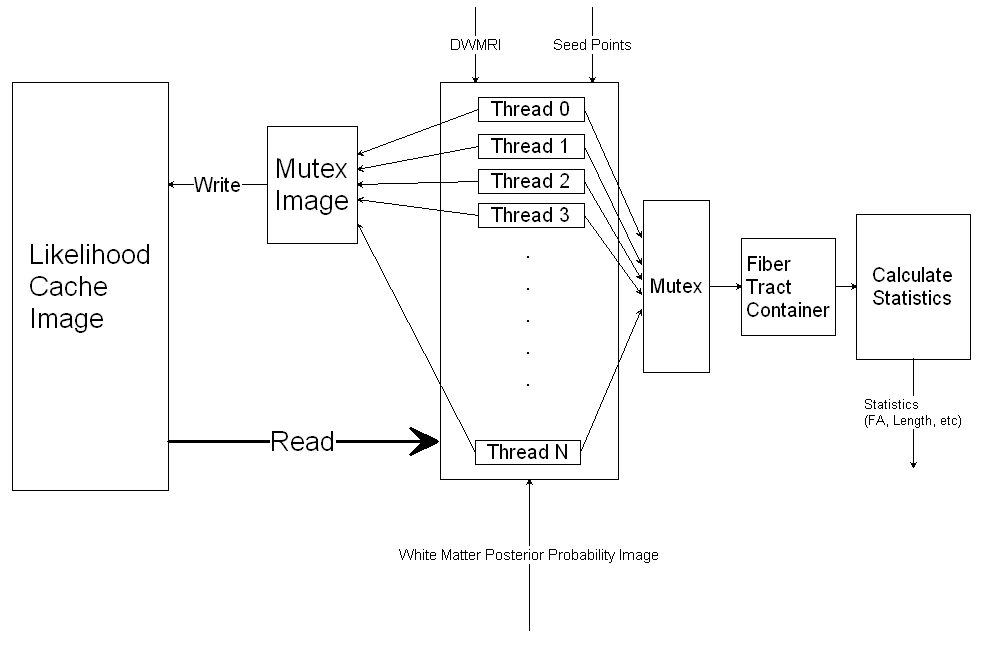
\includegraphics[width=\linewidth]{filterblock}
	\caption{A block diagram of the filter showing its shared likelihood cache and multithreaded architecture.}
	\label{fig:filterblock}
\end{figure}

Each thread of stochastic tractography filter is an instance of the stochastic tractography algorithm. The block diagram in figure \ref{fig:filterblock} demonstrates graphically the architecture of the ITK stochastic tractography filter.  Every thread allocates it own independent memory for the tract that it is currently generating.  Once the tract has terminated, the thread stores a memory pointer to the completed tract in a tract pointer container that is shared among all threads.  The tract pointer container is protected by a mutex, which serializes write operations so that only one thread can store its completed tract in the vector at a time.  Once the filter has generated enough samples, the tracts can be transferred to an output image to create a connectivity map.  Additionally other statistics can be computed on the tracts.  In essence, we divide the process into two sections, a multithreaded portion that samples the tracts and a single threaded portion which accumulates the tracts and calculates relevant statistics on them.

The most computationally expensive part of the algorithm is the calculation of the likelihood distribution.  The algorithm must compute probabilities for 2,562 possible fiber orientations in a voxel.  Fortunately, this likelihood distribution is a deterministic function of the diffusion observations within that voxel.  The filter runs much faster, at the cost of additional memory, by caching the generated likelihood distribution for later access.  Caching is effective because in highly anisotropic regions of the brain, the sampled tracts are expected to be dense causing many of the sampled tracts to visit the same voxels many times.

The cache is implemented as an image whose voxels are re-sizable arrays.  ITK's optimized pixel access capabilities enable quick access to the likelihood distribution associated with any voxel in the image.  On creation, every voxel in the likelihood cache image is initiated to a zero length array.  Whenever the algorithm encounters a voxel, it first checks to see if the likelihood cache contains this voxel by testing if associated array is zero length.  If the voxel has never been visited, the associated array is resized and the computation of the likelihood distribution associated with this voxel is stored inside the newly resized array.

Using a shared likelihood cache between multiple concurrent threads creates additional complexities.  Simultaneous writes to the cache would cause unexpected behavior.  Additionally there is the possibility of one thread reading an incomplete cache entry while another thread is trying to write it.  One possible solution is to ensure that only one thread can read or write to the likelihood cache at a time.  This is easily implemented by serializing access to the likelihood cache using a mutex.  A mutex serves as a lock on data.  A thread will wait to obtain a lock on the data before it proceeds to the next section of code.  Inside this section, which is called the critical section, the thread holds the lock ensuring exclusive access to the otherwise shared data.  All other threads must wait and idle while the thread which owns the lock finishes it operations.  Since threads must access the likelihood cache very often, this results in a situation where many threads are waiting for other threads to finish accessing the likelihood cache.  The serialized access to the likelihood cache creates a bottleneck, which in the worse case would result in performance that is only marginally better than a single threaded version of the filter.
\begin{figure}
  \center
  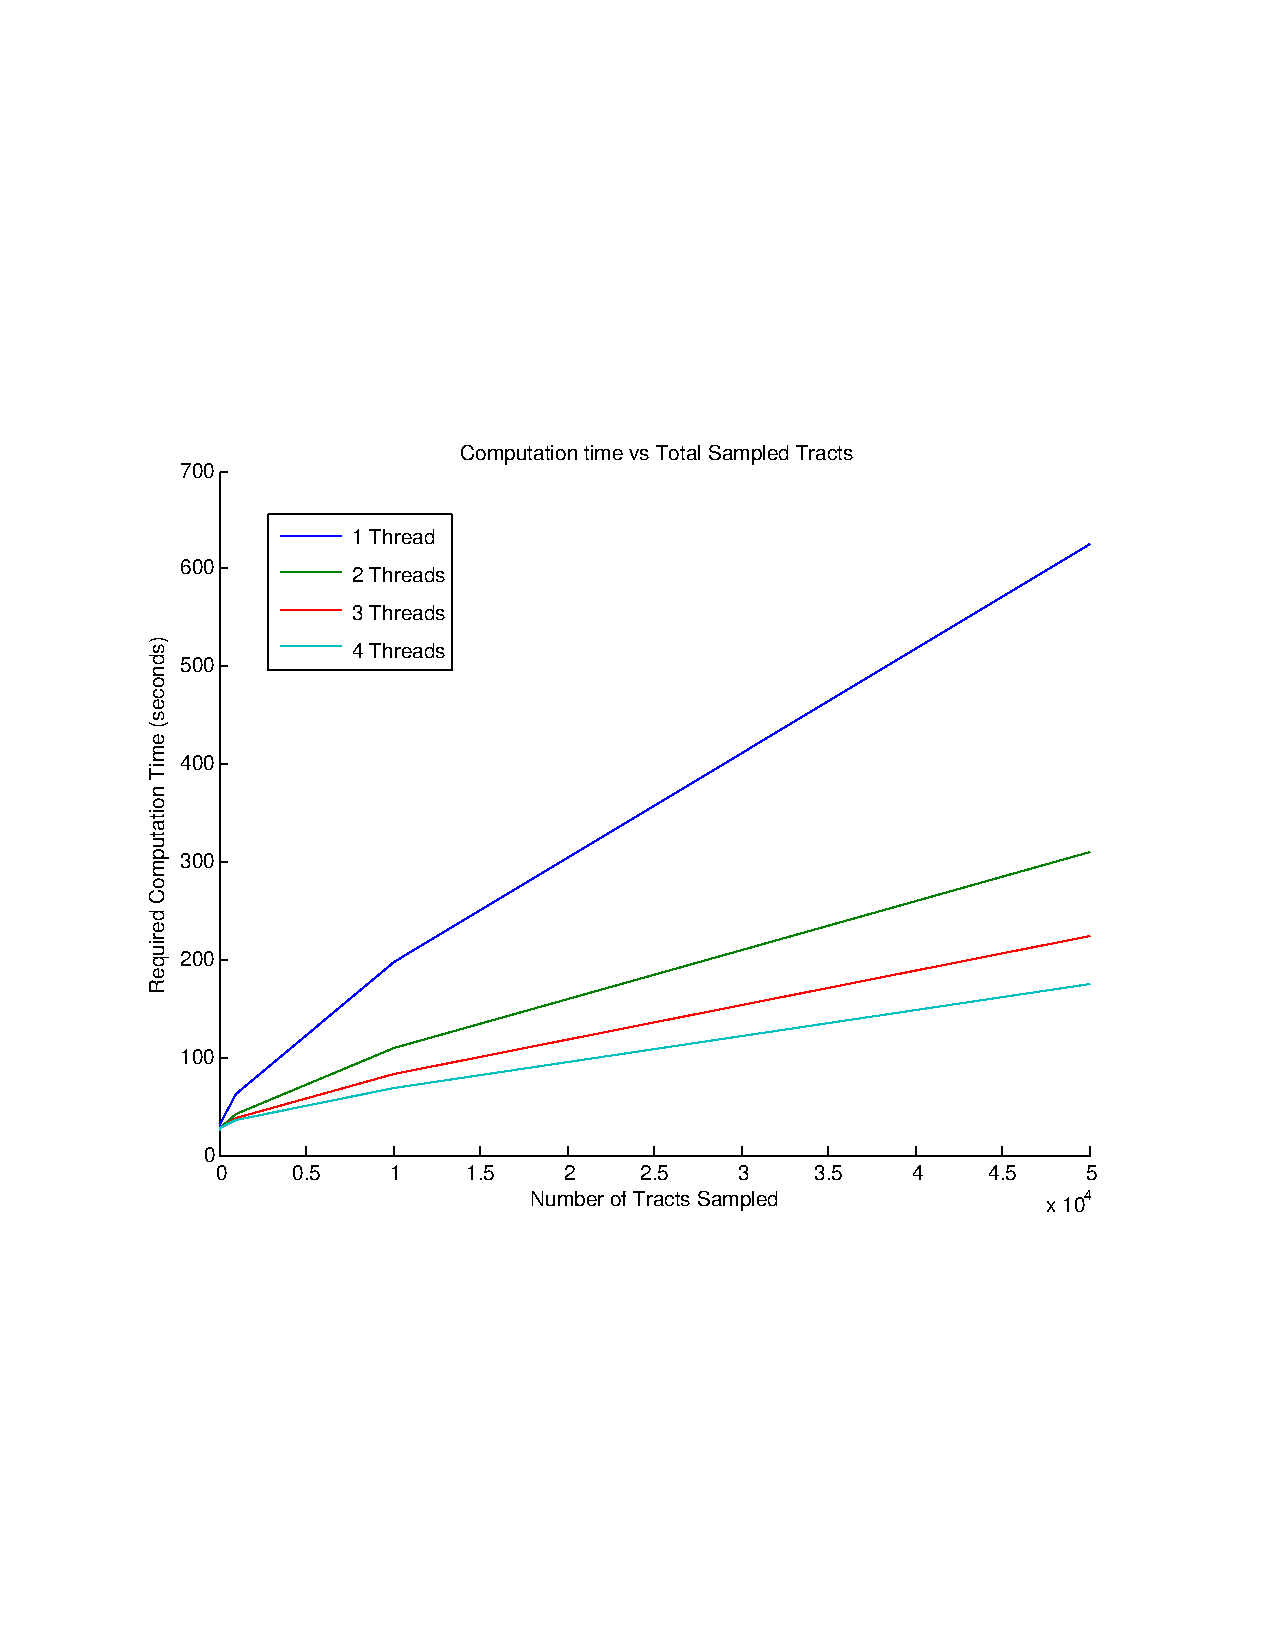
\includegraphics[trim = 20mm 70mm 20mm 70mm, clip, width=0.75\linewidth]
	  {timepertracts}
	\caption{A graph displaying the amount of time needed to sample a number of tracts.  Each line represents the algorithm's performance using different numbers of threads.  This test was run on a 4 processor machine.}
	\label{fig:performance}
\end{figure}

Access collisions to the likelihood cache can be reduced if we increase the granularity of the lock.  Instead of using one large lock for the entire likelihood cache image, we use a lock for each voxel.  The probability of two threads accessing the same voxel simultaneously is much less than the probability of two threads accessing any part of the likelihood cache.  These per voxel locks are conveniently constructed using an ITK image whose voxel data type is a mutex.  Similar to the likelihood cache, this collection of mutexes is indexed by coordinates which correspond to the coordinates of the voxels in the DWI input data.  Again, access to the mutex image is fast due to ITK's optimized access operators for data types indexed by coordinates.  The only cost to using this high resolution mutex image is the additional memory required to store pixel mutexes.  However this cost is small since a mutex is essentially a Boolean variable.  The mutex image allows different voxels in the likelihood cache image to be updated simultaneously, increasing the rate that the likelihood cache is filled.  The advantage of using a mutex image is most evident when tracking in highly isotropic regions,  where collisions are very unlikely to occur, since the sampled paths are very dispersed.  Even on uni-processor systems, using multiple threads may improve performance since the rate of encountering an unvisited voxel may be higher, thus filling the likelihood cache faster. Figure \ref{fig:performance} demonstrates the required computation time for a given number of tracts under different number of threads.

Additionally, to compute the weighted least squares estimates for the log tensor model parameters, we must first estimate the weights.  These weights are found by calculating a least squares estimate of the true intensities of each voxel.  The $\mathbf{A}$ matrix \ref{eq:fulllogtensor} used in this least squares estimation is a function solely of the magnetic gradient directions and associated b-values, which are the same for every voxel in the image.  Since the same $\mathbf{A}$ matrix is used for each voxel in the least squares calculation, a common optimization is to orthogonalize the $\mathbf{A}$ matrix by computing its QR decomposition.  While this operation is computationally expensive, it is performed only once for the entire DWI image.  The orthogonalized $\mathbf{A}$ matrix reduces the cost of computing the weights for every voxel.



\section{User's Guide}

The Stochastic Tractography Filter is implemented as a multithreaded image filter in ITK under the class name itk::StochasticTractographyFilter.  The filter is templated over the DWI and white matter probability map input image types and also on the connectivity map image type.  The filter expects the DWI input image type to be an ITK VectorImage Type.  The code below demonstrates how to instantiate the Stochastic Tractography Filter.
\begin{verbatim}
  //Define Types
  typedef itk::VectorImage< unsigned short int, 3 > DWIVectorImageType;
  typedef itk::Image< float, 3 > WMPImageType;
  typedef itk::Image< unsigned int, 3 > CImageType;
  typedef itk::StochasticTractographyFilter< DWIVectorImageType, WMPImageType,
    CImageType > PTFilterType;
  //Allocate Filter
  PTFilterType::Pointer ptfilterPtr = PTFilterType::New();
\end{verbatim}

The filter's required inputs and parameters must be set before it can be run.  Table \ref{tab:filterinputs} lists filter methods that should be called to set the required inputs and parameters,  and a short description of what each methods expects as arguments.

\begin{table}
  \center
  \begin{tabular}{| l | p{8cm} |}
    \hline 
    \textbf{Filter Member Method} & \textbf{Description}\\
    \hline
    \small{SetInput} & DWI Image: An ITK VectorImage consisting of a vector of DWI measurements including the baseline b0 measurements, at each voxel. \\
    \hline
    \small{SetWhiteMatterProbabilityImageInput} & White Matter Probability Input: An ITK image whose voxel values range from 0 and 1 representing the posterior probability that the voxel is a white matter.  \\
    \hline
    \small{SetbValues} &  b-Values: An ITK VectorContainer whose elements are the corresponding b-values for the DWI input image.  The b0 measurements must have a 0 b-value. \\
    \hline
    \small{SetGradients} & magnetic gradient directions: An ITK VectorContainer whose elements are 3 dimensional vnl vectors.  These vectors should be unit length.\\
    \hline
    \small{SetMeasurementFrame} & DWI Measurement Frame: A 3x3 vnl matrix which transforms the gradient directions to the physical reference frame of the image.  For instance multiplying a magnetic gradient direction vector by the Measurement Frame Matrix will take the vector to the RAS reference frame if RAS is the physical frame of the DWI image. \\
    \hline
    \small{SetMaxTractLength} & Maximum Tract Length: A positive integer that sets the maximum length of a sampled tract.  This can also be interpreted as the number of segments which comprise the tract when using the default step size of 1 unit in the physical frame of the DWI image. \\
    \hline
    \small{SetTotalTracts} & Total Sampled Tracts: A positive integer that sets the total number tracts to sample from the seed voxel. \\
    \hline
    \small{SetMaxLikelihoodCachSize} & Maximum Likelihood Cache Size(MB) A positive integer that sets the maximum size of the Likelihood Cache in megabytes.\\
    \hline
    \small{SetSeedIndex} & Seed Voxel Index:  The discrete index of the seed voxel, in the (IJK) reference frame of the image to start tractography.\\
    \hline
  \end{tabular}
  \caption{ITK Stochastic Tractography Filter Required Inputs and Parameters}
  \label{tab:filterinputs}
\end{table}

The code below is a continuation of the demonstration above and shows how to setup the filter's required inputs and parameters.  The inputs to these methods are provided by ITK's image readers.
\begin{verbatim}
  ptfilterPtr->SetInput( dwireaderPtr->GetOutput() );
  ptfilterPtr->SetWhiteMatterProbabilityImageInput( wmpreader->GetOutput() );
  ptfilterPtr->SetbValues(bValuesPtr);
  ptfilterPtr->SetGradients( gradientsPtr );
  ptfilterPtr->SetMeasurementFrame( measurement_frame );
  ptfilterPtr->SetMaxTractLength( maxtractlength );
  ptfilterPtr->SetTotalTracts( totaltracts );
  ptfilterPtr->SetMaxLikelihoodCacheSize( maxlikelihoodcachesize );
  ptfilterPtr->SetSeedIndex( seedindex );
\end{verbatim}

The filter can then be run by calling the Update method.
\begin{verbatim}
  ptfilterPtr->Update();
\end{verbatim}

For the specified seed voxel, the filter outputs a connectivity map and a container holding all of the sampled tracts used to generate the connectivity map.  The container of sampled tracts can be further processed outside of the stochastic tractography filter to obtain various statistic on the sampled tracts.  Additional seed voxels can be included in the seed region by changing the seed voxel index and rerunning the filter.  The statistics for a multi-voxel seed region can be analyzed by accumulating statistics for all seed voxels within the seed region.  These outputs can be accessed by calling the  \texttt{GetOutput} and  \texttt{GetOutputTractContainer} methods after calling the  \texttt{Update} method.  The code below continues the example above and demonstrates how to obtain the filter's outputs.
\begin{verbatim}
  PTFilterType::TractContainerType::Pointer tractcontainer = 
    ptfilterPtr->GetOutputTractContainer();
  CImageType::Pointer cmap = ptfilterPtr->GetOutput();
\end{verbatim}


%%%%%%%%%%%%%%%%%%%%%%%%%%%%%%%%%%%%%%%%%%%%%%%%%%%%%%%%%%
%
%  Example on how to insert a figure
%
%%%%%%%%%%%%%%%%%%%%%%%%%%%%%%%%%%%%%%%%%%%%%%%%%%%%%%%%%%

%\begin{figure}
%\center
%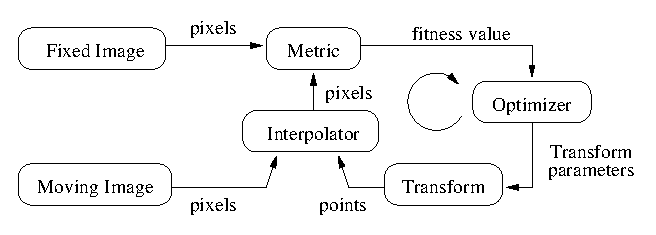
\includegraphics[width=0.8\textwidth]{RegistrationComponentsDiagram.eps}
%\itkcaption[Registration Framework Components]{The basic components of the
%registration framework are two input images, a transform, a metric, an
%interpolator and an optimizer.}
%\label{fig:RegistrationComponents}
%\end{figure}

%%%%%%%%%%%%%%%%%%%%%%%%%%%%%%%%%%%%%%%%%
%
%  Insert the bibliography using BibTeX
%
%%%%%%%%%%%%%%%%%%%%%%%%%%%%%%%%%%%%%%%%%

\bibliographystyle{plain}
\bibliography{InsightJournal}


\end{document}

